\documentclass[arhiv]{../izpit}
\usepackage{fouriernc}
\usepackage{tikz}
\usepackage{censor}
\usepackage{paralist}
\usepackage{listings}

\begin{document}

\izpit{Programiranje I: 4.\ izpit}{4.\ kimavec 2014}{
  Čas reševanja je 150 minut.
  Doseženih 100 točk šteje za maksimalno oceno.
  Veliko uspeha!
}

%%%%%%%%%%%%%%%%%%%%%%%%%%%%%%%%%%%%%%%%%%%%%%%%%%%%%%%%%%%%%%%%%%%%%%
\naloga[Aritmetični izrazi, 10 + 10 + 10 točk]
Aritmetične izraze, kot je na primer
$$(9 * (2 - 7)) + (5 * 3),$$
lahko zapišemo v obliki dvojiškega drevesa (glejte spodnjo sliko). V vsakem vozlišču je zapisano bodisi neko celo število bodisi nek aritmetični operator. (Da ne bi imeli problemov z deljenjem s številom $0$, se bomo omejili na operatorje $+$, $-$ in $*$.) Če vozlišče predstavlja operator, potem ima nujno levega in desnega sina, ki predstavljata ustrezna podizraza. Če vozlišče predstavlja število, je nujno list drevesa. (Ste opazili, da je v korenu drevesa na spodnji sliki operator $+$, ki ga v tem izrazu izračunamo kot zadnjega?)
$$
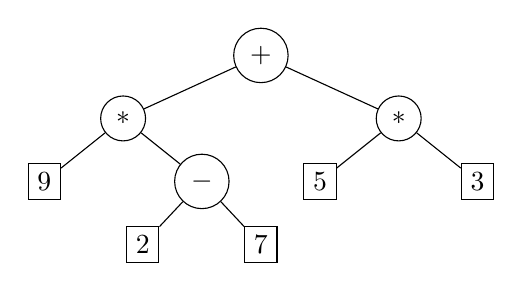
\begin{tikzpicture}[level distance=0.8cm,
    level 1/.style={sibling distance=3.5cm},
    level 2/.style={sibling distance=2cm},
    level 3/.style={sibling distance=1.5cm}
    ]
    \node[circle, draw] (d) {$+$}
      child {node[circle, draw] {$*$}
        child {node[rectangle, draw] {$9$}}
        child {node[circle, draw] {$-$}
          child {node[rectangle, draw] {$2$}}
          child {node[rectangle, draw] {$7$}}
        }
      }
      child {node[circle, draw] {$*$}
        child {node[rectangle, draw] {$5$}}
        child {node[rectangle, draw] {$3$}}
      };
  \end{tikzpicture}
$$
Podatkovna struktura \texttt{Izraz} je že implementirana. Vsako vozlišče ima atribut \texttt{operator}, ki je lahko \verb|'+'|, \verb|'-'|, \verb|'*'| ali \verb|None|. Če je njegova vrednost \verb|None|, predstavlja število in vozlišče ima še atribut \verb+stevilo+ (celo število). Če vrednost atributa \texttt{operator} ni \verb|None|, ima vozlišče še atributa \texttt{levo} in \texttt{desno}, ki predstavljata levi in desni podizraz.

\podnaloga[10 točk]
Sestavite metodo \texttt{naloga1a(self)}, ki izračuna in vrne vrednost tega aritmetičnega izraza. Primer (če \texttt{d} ustreza zgornji sliki):
%
\begin{verbatim}
>>> d.naloga1a()
-30
\end{verbatim}

\podnaloga[10 točk]
Napišite metodo \texttt{naloga1b(self)}, ki vrne niz z običajnim zapisom tega izraza (glejte primer spodaj). Pred in za vsakim operatorjem naj bo po en presledek. Podizrazi naj bodo v oklepajih, razen kadar so le-ti števila. Sicer oklepajev ne smete opuščati (pa čeprav nam asociativnostni zakon to omogoča). Primer (če \texttt{d} ustreza zgornji sliki):
%
\begin{verbatim}
>>> d.naloga1b()
'(9 * (2 - 7)) + (5 * 3)'
\end{verbatim}

\podnaloga[10 točk]
Sestavite metodo \texttt{naloga1c(self)}, ki izraz poenostavi, tako da odpravi ``najbolj notranje'' operatorje, tj.\ tiste
operatorje, kjer sta oba podizraza števili. Primer (če \texttt{d} ustreza zgornji sliki):
%
\begin{verbatim}
>>> d.naloga1c()
>>> d
Izraz('+', levo=Izraz('*', levo=Izraz(9), desno=Izraz(-5)), desno=Izraz(15))
\end{verbatim}
$$
%
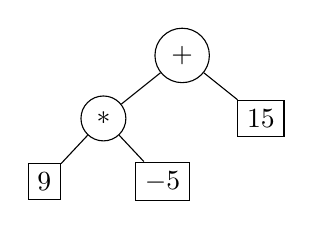
\begin{tikzpicture}[level distance=0.8cm,
    level 1/.style={sibling distance=2cm},
    level 2/.style={sibling distance=1.5cm},
    ]
    \node[circle, draw] (d) {$+$}
      child {node[circle, draw] {$*$}
        child {node[rectangle, draw] {$9$}}
        child {node[rectangle, draw] {$-5$}}
      }
      child {node[rectangle, draw] {$15$}};
  \end{tikzpicture}
$$

%%%%%%%%%%%%%%%%%%%%%%%%%%%%%%%%%%%%%%%%%%%%%%%%%%%%%%%%%%%%%%%%%%%%%%
\naloga[Risanje grafov s paketom TikZ, 15 + 20 točk]

Pri tej nalogi bomo spoznali, kako narišemo graf v \LaTeX u z uporabo paketka TikZ. Risali bomo
samo takšne slike, kjer bodo povezave \emph{ravne črte}. Graf podamo z:
\begin{compactitem}
\item slovarjem \texttt{vozlisca}, kjer so ključi oznake vozlišč, vrednosti pa njihove koordinate;
\item seznamom povezav \texttt{povezave}.
\end{compactitem}
%
Graf na spodnji sliki bi torej podali takole:
\begin{verbatim}
vozlisca_1 = {0: (0, 0), 1: (0, 1), 2: (1, 0), 3: (1, 1), 4: (1.87, 0.5)}
povezave_1 = [(0, 1), (2, 3), (2, 4), (3, 4)]
\end{verbatim}
%
$$
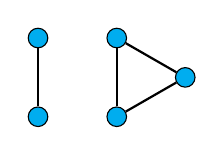
\begin{tikzpicture}
\tikzstyle{every node} = [draw, thin, fill=cyan, circle, inner sep=2.5pt]
\tikzstyle{every path} = [draw, thick]
\node (v_0) at (0, 0) {};
\node (v_1) at (0, 1) {};
\node (v_2) at (1, 0) {};
\node (v_3) at (1, 1) {};
\node (v_4) at (1.87, 0.5) {};
\path (v_0) -- (v_1);
\path (v_2) -- (v_3);
\path (v_3) -- (v_4);
\path (v_2) -- (v_4);
\end{tikzpicture}
$$
%
Ta slika je narisana v TikZ in sicer z naslednjimi ukazi:
\begin{verbatim}
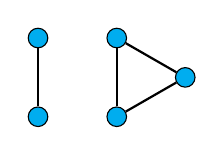
\begin{tikzpicture}
\tikzstyle{every node} = [draw, thin, fill=cyan, circle, inner sep=2.5pt]
\tikzstyle{every path} = [draw, thick]
\node (v_0) at (0, 0) {};
\node (v_1) at (0, 1) {};
\node (v_2) at (1, 0) {};
\node (v_3) at (1, 1) {};
\node (v_4) at (1.87, 0.5) {};
\path (v_0) -- (v_1);
\path (v_2) -- (v_3);
\path (v_3) -- (v_4);
\path (v_2) -- (v_4);
\end{tikzpicture}
\end{verbatim}

\podnaloga[15 točk]
Sestavite funkcijo \texttt{tikz(vozlisca, povezave)}, ki kot argumenta dobi slovar in seznam, kot sta opisana zgoraj. Funkcija naj vrne niz, ki vsebuje TikZ kodo, ki nariše to sliko.

Oznake vozlišč bodo celoštevilske. Za vsako vozlišče mora biti v kodi po eno vrstica oblike
\begin{lstlisting}[basicstyle=\ttfamily]
\node (v_Q) at (X, Y) {};
\end{lstlisting}
kjer je namesto \texttt{Q} oznaka vozlišča, namesto \texttt{X} in \texttt{Y} pa koordinati vozlišča. Vrstice naj bodo urejene glede na oznake vozlišč. Za vsako povezavo iz seznama \texttt{povezave} mora biti v kodi po ena vrstica oblike
\begin{lstlisting}[basicstyle=\ttfamily]
\path (v_Q) -- (v_W);
\end{lstlisting}
kjer sta namesto \texttt{Q} in \texttt{W} oznaki vozlišč. Glava in noga sta fiksni (in sta tudi že definirani v preambuli).
Primer (spremenljivki \texttt{vozlisca\_1} in \texttt{povezave\_1} sta podani zgoraj):
%
\lstset{basicstyle=\ttfamily,breaklines=true}
\begin{verbatim}
>>> tikz(vozlisca_1, povezave_1)
'\\begin{tikzpicture}\n\\tikzstyle{every node} = [draw, thin, fill=cyan, circle, 
inner sep=2.5pt]\n\\tikzstyle{every path} = [draw, thick]\n\\node (v_0) at (0, 0)
 {};\n\\node (v_1) at (0, 1) {};\n\\node (v_2) at (1, 0) {};\n\\node (v_3) at (1,
 1) {};\n\\node (v_4) at (1.87, 0.5) {};\n\\path (v_0) -- (v_1);\n\\path (v_2) --
 (v_3);\n\\path (v_2) -- (v_4);\n\\path (v_3) -- (v_4);\n\\end{tikzpicture}'
\end{verbatim}
%
\podnaloga[20 točk] Sestavite še funkcijo \texttt{preberi\_graf(koda)}, ki kot argument dobi niz s TikZ kodo. Funkcija naj vrne slovar in seznam, kot sta definirana zgoraj.
Primer (v spremenljivki \texttt{tikz\_koda} naj bo niz iz primera zgoraj):
%
\begin{verbatim}
>>> preberi_graf(tikz_koda)
({0: (0.0, 0.0), 1: (0.0, 1.0), 2: (1.0, 0.0), 3: (1.0, 1.0), 4: (1.87, 0.5)},
 [(0, 1), (2, 3), (2, 4), (3, 4)])
\end{verbatim}
%
Predpostavite lahko, da bo \texttt{koda} vedno lepo oblikovana, tako kot je na primeru zgoraj.
%

%%%%%%%%%%%%%%%%%%%%%%%%%%%%%%%%%%%%%%%%%%%%%%%%%%%%%%%%%%%%%%%%%%%%%%
\naloga[Igra življenja, 20 + 5 točk]

Pri igri življenja svet predstavimo s pravokotno matriko, katere elementi so števila iz množice $\{0, 1\}$. Število 0 predstavlja \emph{mrtvo} celico, število 1 pa predstavlja \emph{živo} celico. Osem celic, ki obdajajo izbrano celico matrike, imenujemo \emph{sosedje}. (Robne celice imajo manj kot 8 sesedov, če smo povsem natančni.) Igra življenja poteka v diskretnih časovnih korakih. Pravila so naslednja:
\vspace{\baselineskip}

\begin{compactitem}
\item Živa celica, ki ima manj kot 2 živa soseda, umre (osamljenost).
\item Živa celica, ki ima več kot 3 žive sosede, umre (prenaseljenost).
\item Živa celica, ki ima 2 ali 3 žive sosede, preživi.
\item Mrtva celica, ki ima natanko 3 žive sosede, oživi (reprodukcija).
\end{compactitem}

\podnaloga[20 točk]
\noindent V \emph{Mathematici} sestavite funkcijo \texttt{zivljenje[svet\_]}, ki kot argument dobi matriko, ki pred\-stav\-lja svet, in vrne novo matriko, ki predstavlja novi svet po enem koraku igre življenja. Primer:
%
\begin{verbatim}
In[1]:= svet = {{0, 1, 0, 1}, {1, 0, 1, 0}, {1, 0, 0, 0}, {0, 0, 0, 1}};
In[2]:= zivljenje[svet]
Out[2]= {{0, 1, 1, 0}, {1, 0, 1, 0}, {0, 1, 0, 0}, {0, 0, 0, 0}}
\end{verbatim}

\podnaloga[5 točk]
Ugotovite, koliko korakov je potrebno narediti v igri življenja, da svet \texttt{dieHard} izumre. Svet \texttt{dieHard} je že definiran v zvezku. Lahko si pomagate tudi s funkcijo \texttt{Manipulate}, ki jo prav tako najdete v zvezku.

%%%%%%%%%%%%%%%%%%%%%%%%%%%%%%%%%%%%%%%%%%%%%%%%%%%%%%%%%%%%%%%%%%%%%%
\naloga[Krogi, 30 točk]

V \emph{Mathematici} sestavite funkcijo \texttt{krogi[l\_]}, ki nariše kroge, kakor je prikazano na slikah spodaj. Kot argument funkcija dobi poljubno dolg seznam celih števil \texttt{l}, ki sme vsebovati le cela števila 0, 1 in 2.

Osnovni vzorec, ki ga bomo imenovali \emph{grozd}, je sestavljen iz treh enako velikih krogov, ki se medsebojno dotikajo (spodnja dva sta horizontalno poravnana, tretji pa je postavljen nad njima). Nato si izberemo enega od krogov in mu včrtamo grozd. V malem grozdu spet izberemo enega od krogov in mu včrtamo grozd itd. Kateri grozd je potrebno izbrati na vsakem koraku, nam povedo števila v seznamu \texttt{l}. Število 0 pomeni zgornjega, 1 pomeni spodnjega levega, 2 pa spodnjega desnega.

\begin{center}
\begin{tabular}{c@{\hspace{0.5cm}}c@{\hspace{0.5cm}}c}
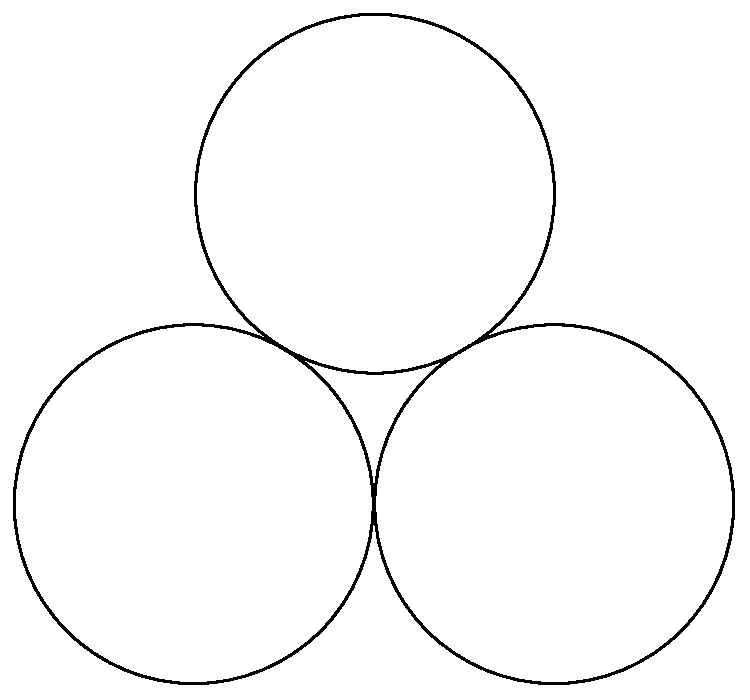
\includegraphics[width=5cm]{krogi-prazen.pdf}&
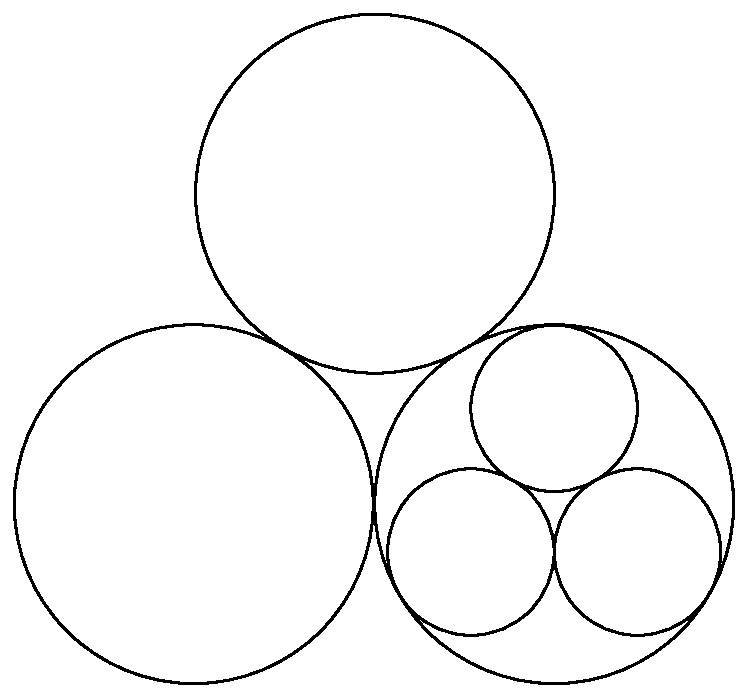
\includegraphics[width=5cm]{krogi-2.pdf}&
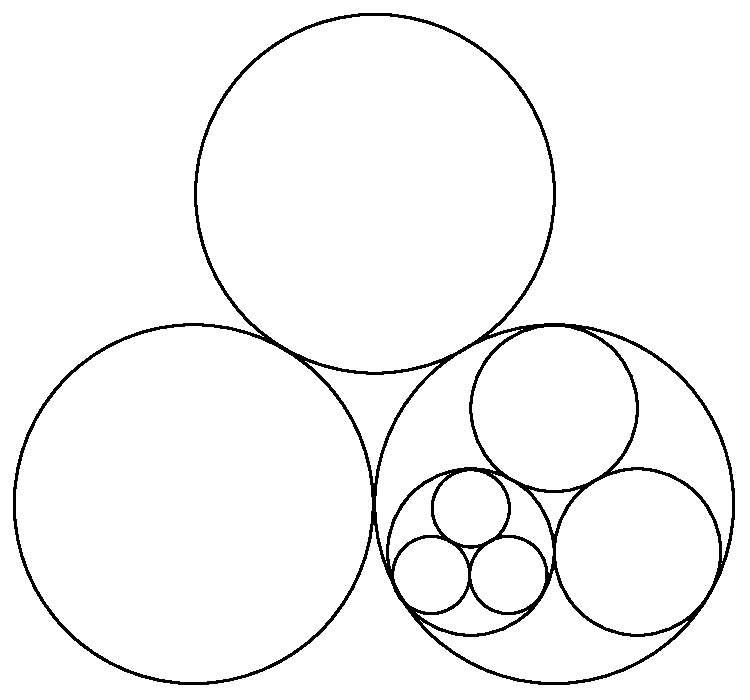
\includegraphics[width=5cm]{krogi-21.pdf}\\
\texttt{krogi[\{\}]} &
\texttt{krogi[\{2\}]} &
\texttt{krogi[\{2, 1\}]}
\end{tabular}
\end{center}
\end{document}
